%%%%%%%%%%%%%%%%%%%%%%% file typeinst.tex %%%%%%%%%%%%%%%%%%%%%%%%%
%
% This is the LaTeX source for the instructions to authors using
% the LaTeX document class 'llncs.cls' for contributions to
% the Lecture Notes in Computer Sciences series.
% http://www.springer.com/lncs       Springer Heidelberg 2006/05/04
%
% It may be used as a template for your own input - copy it
% to a new file with a new name and use it as the basis
% for your article.
%
% NB: the document class 'llncs' has its own and detailed documentation, see
% ftp://ftp.springer.de/data/pubftp/pub/tex/latex/llncs/latex2e/llncsdoc.pdf
%
%%%%%%%%%%%%%%%%%%%%%%%%%%%%%%%%%%%%%%%%%%%%%%%%%%%%%%%%%%%%%%%%%%%


\documentclass[runningheads,a4paper]{llncs}

\usepackage{amssymb}
\setcounter{tocdepth}{3}
\usepackage{graphicx}
%%%%%%%%%%%%%%% New package
\usepackage{amsmath}
\usepackage{caption}
\usepackage{subfig}
\usepackage{csvsimple}
\usepackage{multirow}
\usepackage{array}
\usepackage{booktabs}
%%%%%%%%%%%%%%%
\usepackage{url}
% \urldef{\mailsa}\path|{soltanin, locheng, ingrid.haas, frank.holzwarth,|
% \urldef{\mailsb}\path|anna.kramer, leonie.kunz, christine.reiss, nicole.sator,|
% \urldef{\mailsc}\path|erika.siebert-cole, peter.strasser, lncs}@springer.com|
% \newcommand{\keywords}[1]{\par\addvspace\baselineskip
% \noindent\keywordname\enspace\ignorespaces#1}

\begin{document}

%\mainmatter  % start of an individual contribution

% first the title is needed
\title{Towards the identification of Parkinson’s Disease using only T1 MR Images}

% a short form should be given in case it is too long for the running head
%\titlerunning{Lecture Notes in Computer Science: Authors' Instructions}

% the name(s) of the author(s) follow(s) next
%
% NB: Chinese authors should write their first names(s) in front of
% their surnames. This ensures that the names appear correctly in
% the running heads and the author index.
%
\author{Sara Soltaninejad\and Irene Cheng\and Anup Basu}
%\thanks{Please note that the LNCS Editorial assumes that all authors have used
%the western naming convention, with given names preceding surnames. This determines
%the structure of the names in the running heads and the author index.}%

%%
%\authorrunning{Lecture Notes in Computer Science: Authors' Instructions}
% (feature abused for this document to repeat the title also on left hand pages)

% the affiliations are given next; don't give your e-mail address
% unless you accept that it will be published
\institute{Dept. of Computing Science, University of Alberta, Canada}

%
% NB: a more complex sample for affiliations and the mapping to the
% corresponding authors can be found in the file "llncs.dem"
% (search for the string "\mainmatter" where a contribution starts).
% "llncs.dem" accompanies the document class "llncs.cls".
%

% \toctitle{Lecture Notes in Computer Science}
% \tocauthor{Authors' Instructions}
\maketitle


\begin{abstract}
Parkinson’s Disease (PD) is one of the most common type of neurological disease caused by progressive degeneration of dopaminergic neurons in the brain. Even though there is no fixed cure for this neurodegenerative disease, earlier diagnosis and resulting earlier treatment can help patients have better quality of life. Magnetic Resonance Imaging (MRI) is one of the most popular means of diagnosis in recent years because it avoids harmful radiations. In this paper, we investigate the plausibility of using MRIs for automatically diagnosing PD. Our proposed method has three main steps : 1) Preprocessing, 2) Feature Extraction, and 3) Classification. The Fressurfer library is used for the first and second steps. For classification, three main types of the classifiers, including Logistic Regression (LR), Random Forest (RF) and Support Vector Machine (SVM) are applied and their classification ability is compared. The Parkinson’s
Progression Markers Initiative (PPMI) data set is used for evaluation of the proposed method. The proposed system is shown to be promising in assisting the diagnosis of PD.
\end{abstract}


\section{Introduction}
Parkinson's Disease (PD) is the second most important neurodegenerative disease after Alzheimer's Disease (AD) that affects middle age and elderly people. The statistical information presented by Parkinson’s News Today \cite{1} shows that an estimated seven to ten million people worldwide have Parkinson’s disease. PD causes progressive loss of dopamine generating neurons in the brain resulting in two types of symptoms, including motor and non-motor. The motor symptoms are bradykinesia, muscles rigidity, tremor and abnormal gait \cite{2} whereas non-motor symptoms show mental disorders, sleep problems and sensory disturbance \cite{3}.
Even though there are some medical methods for diagnosing and progress determination of PD, the results from these experiments are subjective and depends on the expertise of the clinicians. On the other hand, clinicians are expensive and the process is time consuming for the patients \cite{4}. Neuroimaging techniques have significantly improved the diagnosis of neurodegenerative  diseases. There are different types of neuro imaging techniques of which Magnetic Resonance Imaging (MRI) is one of the most popular one because it is a cheap and non-invasiveness method. People with PD show their symptoms when they lose almost $80\%$ of their brain dopamine \cite{5}. All of these facts prove the urgent need to have a Computer Aided Diagnosis (CAD) system for automatic detection of this type of disease.
In recent years machine learning has shown remarkable results in the medical image analysis field. The proposed CAD system in neuro disease diagnosis uses different types of imaging data including Single-Photon Emission Computed Tomography (SPECT) (Prashanth et al. \cite{6}), DTI, Positron Emission Tomography (PET)(Loane and Politis \cite{7}) and MRI. In this study, the goal is to utilize structural MRI (sMRI) for developing automated CAD for early diagnosis of PD. Focke et al. \cite{8} proposed a method for PD classification using MR Images. The proposed method in \cite{8} used Gray Matter (GM) and White Matter (WM) individually with an SVM classifier. Voxel-based morphometry (VBM) has been used for preprocessing and feature extraction. The reported results show poor performance 39.53\% for GM and 41.86\% for WM. In \cite{9} Babu et al. proposed a CAD system for diagnosing PD. Their method has three general steps: feature extraction, feature selection and classification. In the first part the VBM is used over GM to construct feature data. For the feature selection, recursive feature elimination (RFE) was used to select the most discriminative features. In the last step,  projection based learning and meta-cognitive radial basis function was used for classification, which resulted in 87.21\% accuracy. The potential biomarker for PD is identified as the superior temporal gyrus. The limitation in this work is that VBM is univariate and RFE is computationally expensive.
Salvatore et al. \cite{9}, proposed a method that used PCA for feature extraction. The PCA was applied on normalized skull stripped MRI data. Then, SVM was used as the classifier, giving 85.8\% accuracy.
Rana et al. \cite{10} extracted features over the three main tissues of the brain consisting of WM, GM and CSF. Then, they used t-test for feature selection and in the next step SVM for classification. This resulted in 86.67\% accuracy for GM and WM and 83.33\% accuracy for CSF. In their other work \cite{11},  graph-theory based spectral feature selection method was applied to select a set of discriminating features from the whole brain volume. A decision model was built using SVM as a classifier with a leave-one-out cross-validation scheme, giving 86.67\% accuracy. The proposed method in \cite{4} was not focused on just individual tissues (GM,WM and CSF) but it considered the relationship between these areas because the morphometric change in one tissue might affect other tissues. $3D$ LBP was used as a feature extraction tool which could produce structural and statistical information. After that, minimum redundancy and maximum relevance with t-test are used as feature selection methods to get the most discriminative and non-redundant features. In the end, SVM is used for classification which gives 89.67\% accuracy.
In \cite{13}, the low level features (GM, cortical volume, etc.) and the high level features (region of interest (ROI) connectivity) are combined to perform a multilevel ROI feature extraction. Then, filter and wrapper feature selection method is followed up with multi kernel SVM to achieve 85.78\% accuracy for differentiation of PD and healthy control (HC) data.
Adeli et al. \cite{14} proposed a new joint feature-sample selection (JFSS) procedure, which jointly selects the best subset of the most discriminative features and the best sample to build a classification model. Experimental results on both synthetic and publicly available PD datasets show promising results.

In our paper, a CAD system is presented for diagnosing of PD by using only MR T1 images. Our goal is to avoid other modalities, like PET etc., that expose patients to harmful radiation. The general steps of the proposed method is shown in Fig.\ref{fig:framework} and includes preprocessing, feature extraction and classification.

The remaining sections of this paper are structured as follows: Section 2 and 3 covers materials and methods, which provides details on the dataset, preprocessing and the proposed method for PD classification. Experimental results and discussion are covered in Section 4. Finally, Section 5 presents the conclusion.


\section{Data Set}
The data used in the preparation of this article is the T1-weighted brain MR images obtained from the PPMI database \url{www.ppmi-info.org/data}. For up-to-date information on the study please visit \url{www.ppmiinfo.org}. PPMI is a landmark, large-scale, international and multi-center study to identify PD progression biomarkers \cite{15}. The data that is used in our study contains the original T1 MR image of $598$ samples with $411$ PD and $187$ Control. Furthermore, it contains demographic or clinical information on the age and sex of the subjects. The summary of the data base is presented in Table \ref{tab:ppmi}. Based on the demographic information in this table, the balance of dataset is presented for the two type of classes which are Parkinson disease (PD) and healthy control (HC).
\begin{table}[h]\small
  \centering
  \caption{Demographics of the PPMI}
  \begin{tabular}{|>{\bfseries}c|*{7}{c|}}\hline
    \multirow{2}{*}{\bfseries Data Type}
    & \multicolumn{2}{c|}{\bfseries Class}
    &\multicolumn{2}{c|}{\bfseries Sex}
    & \multicolumn{3}{c|}{\bfseries Age} \\\cline{2-8}
    & \textbf{PD} & \textbf{HC} & \textbf{F}&\textbf{M} & \textbf{(25-50)}&\textbf{(50-76)} &\textbf{(75-100)}\\ \hline
           Number of Subjects   &411 & 187 & 217 & 381 & 81&472&45      \\ \hline
  \end{tabular}
  \label{tab:ppmi}
\end{table}



% \begin{table}[]
% \centering
% \caption{PPMI Database Information}
% \label{tab:ppmi}
% \begin{tabular}{|l|l|l|l|l|l|l|l|}
% \hline
%                  & PD  & NC & F  & M   & Age (25-50)& Age (50-76)& Age (75-100)    \\ \hline
% PPMI & 411 & 187 & 217 & 381 & 81&472&45 \\ \hline
% \end{tabular}
% \end{table}
% \begin{figure}
% \centering
% 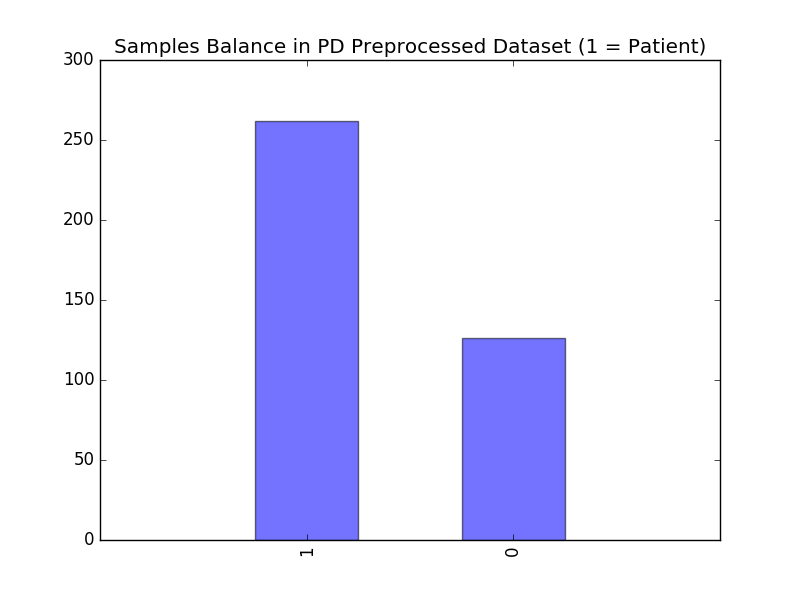
\includegraphics[scale=0.4]{dbal.png}
% \caption{Dataset balance for two class of PD and HC.}
% \label{fig:dbal}
% \end{figure}
% After downloading the data, the real information is as below:\\
% \begin{itemize}
% \item total number of subjects are = 568
% \item number of PD subjects = 390
% \item number of NC subjects = 178
% \end{itemize}

\section{Proposed Method}
The overview of our proposed method is presented in Fig.\ref{fig:framework}  which has $3$ general steps including: 1- Preprocessing; 2- Feature Extraction; and 3- Classification. Next, each step is explained in detail. The goals of CAD system goals are:
\begin{enumerate}
\item Extracting the volume based features from the MR T1 images using the automated surface-based analysis package FreeSurfer.
\item Comparing the capability of different types of classifiers for diagnosing PD.
\end{enumerate}

\begin{figure}[h!]
%\centering
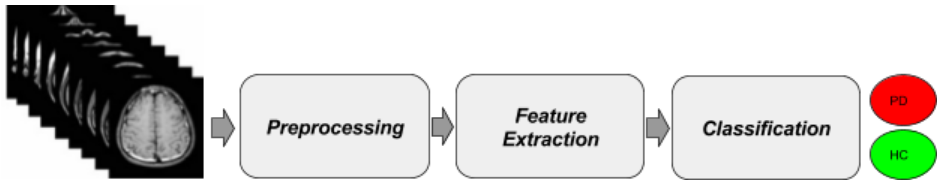
\includegraphics[scale=0.37]{flchart.png}
\caption{The general framework of the proposed methods.}
\label{fig:framework}
\end{figure}
\subsection{Preprocessing}
Preprocessing is an essential step in designing the CAD system which provides informative data for the next steps. In this paper, for computing the volumetric information of the MRI subject’s, several preprocessing steps are needed. The Freesurfer image analysis suite is used for performing preprocessing over the 3D MRI data. FreeSurfer is a software package for the analysis and visualization of structural and functional neuroimaging data from cross-sectional or longitudinal studies \cite{16}. The FreeSurfer pipeline performs cortical reconstruction and subcortical volumetric segmentation including the removal of non-brain tissue (skull, eyeballs and skin), using an automated algorithm with the ability to successfully segment the whole brain without any user intervention \cite{f}. FreeSurfer is the structural MRI analysis software of choice for the Human Connectome Project which is documented and freely available for download on-line (http://surfer.nmr.mgh.harvard.edu/). In total 31 preprocessing steps has completed using FreeSurfer, of which some are shown in Fig.\ref{fig:prepsteps}.
\begin{figure}
\centering
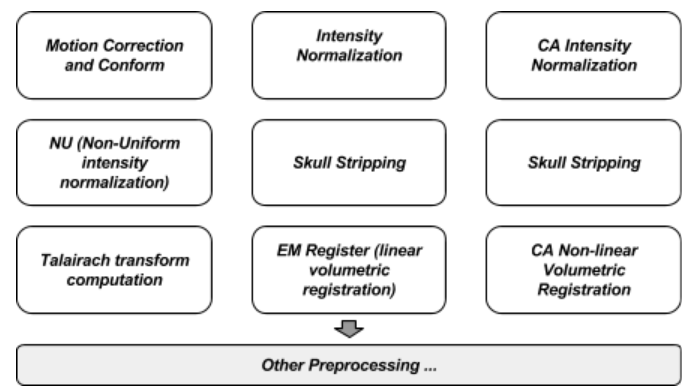
\includegraphics[scale=0.4]{Preprocessing.png}
\caption{Preprocessing steps.}
\label{fig:prepsteps}
\end{figure}

There are two types of failures in the preprocessing step which can be categorized into hard failure and soft failure. Hard failures are related to the subjects for whom preprocessing is not successful and the soft failure are related to the subjects that are preprocessed but there are some problem in the results of preprocessing. Out of $568$ subjects MRIs, $388$ images were successfully preprocessed. Other images were excluded from
the dataset due to poor quality of the original images
or unknown CDR labels.

\subsection{Feature Extraction}
After preprocessing using FreeSurfer, a list of volume based features are extracted from different regions of the brain. These features are captured from the regions segmented by brain parcellation using FreeSurfer. Some of the features collected in the left and right hemispheres of the brain are listed below:
\begin{enumerate}
	\item Left and right lateral ventricle
	\item Left and right cerebellum white matter
	\item Cerebrospinal fluid (CSF)
	\item Left and right hippocampus
	\item left and right hemisphere cortex
	\item Estimated total intra cranial (eTIV)
	\item left and right hemisphere surface holes
\end{enumerate}
The extracted feature data is based on Equation \ref{eq:fd}.
\begin{equation}
FeatureData =
\begin{bmatrix}
    f_{11}       & f_{12} & f_{13} & \dots & f_{1n} \\
    f_{21}       & x_{22} & x_{23} & \dots & f_{2n} \\
    %\hdotsfor{5} \\
    \qquad \ldots\\
    f_{s1}       & f_{s2} & f_{s3} & \dots & f_{sn}
\end{bmatrix}
%FeatureData = [f_{i,j}] \quad i \in [1:n], j\in [1:m]\\
\label{eq:fd}
\end{equation}
Where $s$ is the number of subjects and $n$ is the number of extracted features for that subject. In this study, $n$ is $388$ and $m$ is $139$.

Furthermore, there are two other type of features which are provided by the PPMI dataset which are age and sex for each subject. Thus, these two biographical information could be added to the extracted feature which gives feature data with the size $(388*141)$.
\subsection{Classification}
In this part the aim is using the extracted volume based features for classifying the MRI data into two classes of PD and HC. In our study, three types of supervised classification algorithm are used. Next, each classification method is described:
\begin{itemize}
\item \textbf{Logistic Regression (LR):}\\
Logistic regression (LR) is a statistical technique which is used in machine learning for binary classification problems. LR belongs to the family of MaxEnt classifiers known as the exponential or log-linear classifiers \cite{LR}. Like naive Bayes, it works by extracting some set of weighted features from the input, taking logs, and combining them linearly (meaning that each feature is multiplied by a weight and then added up) \cite{17}. Thus, this model is a suitable binary classifier for our problem.
\item \textbf{Random Forest (RF):}\\
Random forests (RF) is an ensemble learning method for classification, regression and other tasks. This method is presented by Breiman \cite{18}, which creates a set of decision trees from a randomly selected subset of training data. It then aggregates the votes from different decision trees to define final class of the test object. Each tree in a random forest is a weak classifier. A large set of trees trained with randomly chosen data makes a single decision on a majority basis. In the current stage of this research, we tested how accurate decisions can be made by random forests trained by the data coming from a single MRI volume.
\item \textbf{Support Vector machine (SVM):} \\
Support vector machine (SVM) \cite{19} is a well-known supervised machine learning algorithm for classification and regression. It performs classification tasks by constructing optimal hyperplanes in a multidimensional space that separates cases of different class labels. This classification method is more popular because it is easier to use, has higher generalization performance and less tuning comparing to other classifiers. In our case, the kernel SVM is used.

\end{itemize}

There is a set of parameters for each classifier that needs to be tuned in order to have a fair comparison.

\section{Results and Discussion}
In this section, the experimental results for different steps of the proposed CAD system for diagnosis of PD is presented. First the preprocessing step prepares the MRI data for the next steps using FreeSurfer. Fig.\ref{fig:prepres} shows the MRI for subject $3102$ and the resulting image after preprocessing.

\begin{figure}[!h]\small
  \centering
  \subfloat[Original MR image.]{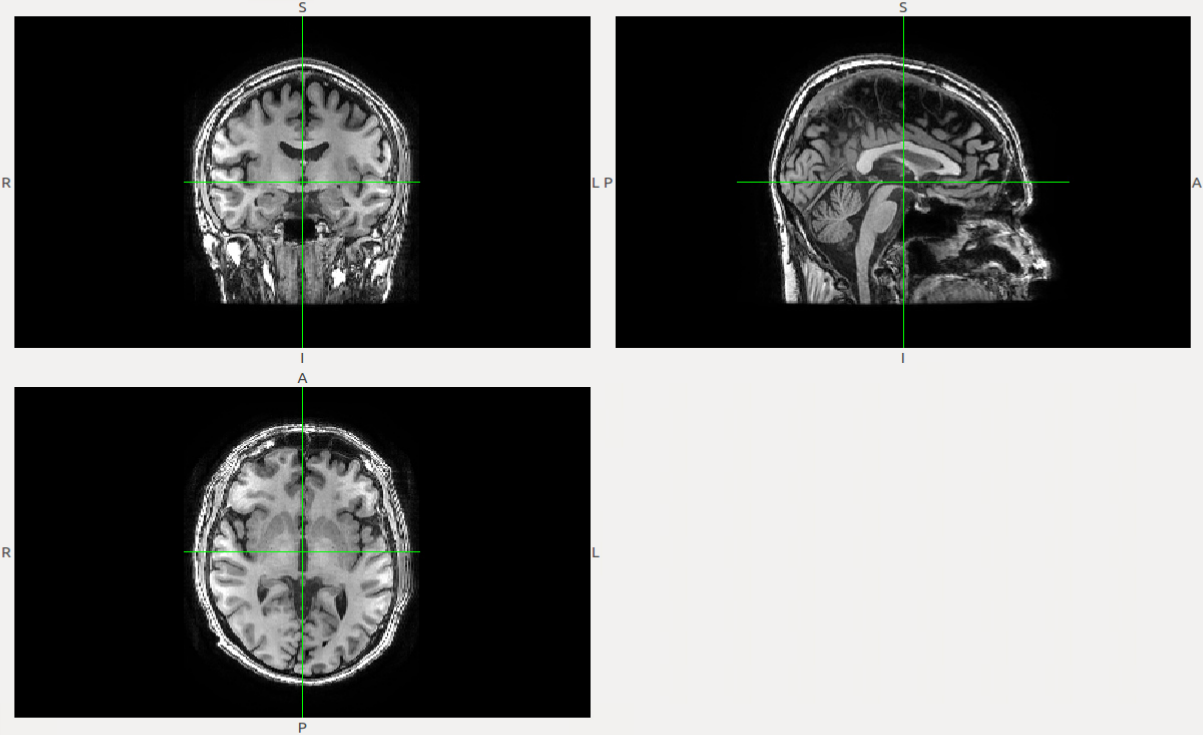
\includegraphics[scale=0.25]{orgimg.png}\label{fig:f1}}%[width=0.5\textwidth]
  \hfill
  \subfloat[Preprocessed MR image.]{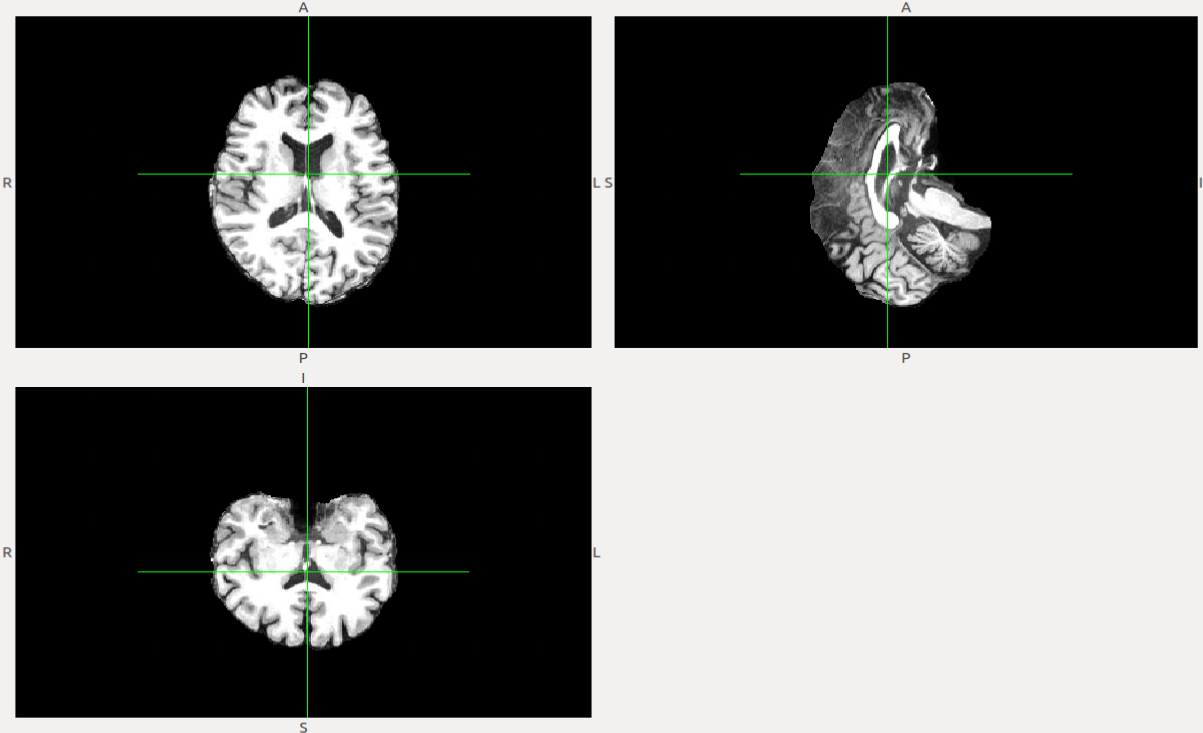
\includegraphics[scale=0.25]{prep.png}\label{fig:f2}}
  \caption{Preprocessing results for one of the subjects.}
  \label{fig:prepres}
\end{figure}
After preprocessing with FreeSurfer, for each subject a list of volume-based features is extracted. Also, age and sex are provided for the PPMI data in their website as demographic information of the patients. Some evaluation has been done over the set of extracted features in terms of their discrimination ability. Since PD is an age related disease, the distribution of data in terms of age feature is plotted. Fig.\ref{fig:agelabel} shows the distribution of age in the dataset for the subjects with PD and HC labels.
\begin{figure}[h]\small
\centering
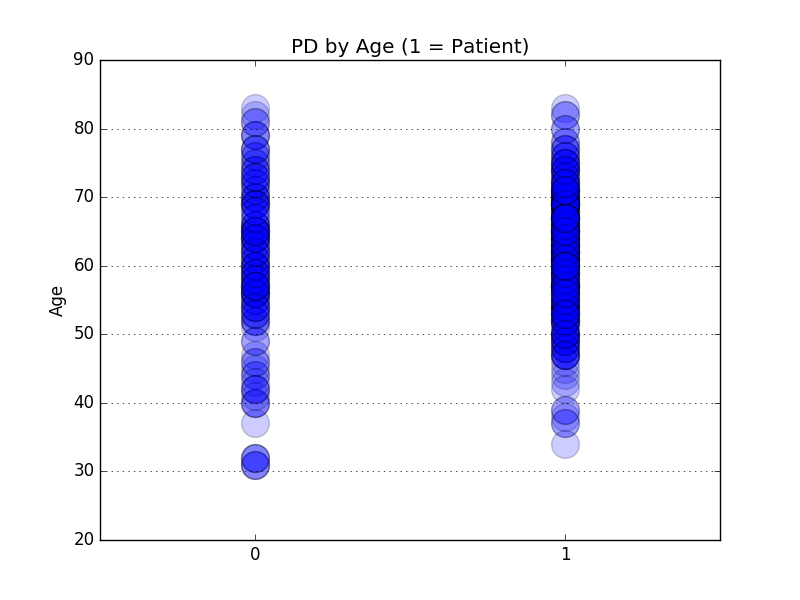
\includegraphics[scale=0.4]{AgeData.png}
\caption{Distribution of Data in terms of Age feature.}
\label{fig:agelabel}
\end{figure}
The distribution of all the extracted features are plotted in terms of their ability to distinguish the data into two classes of PD and HC. Some of these distributions are shown in Fig.\ref{fig:feateval}. As can be seen in Fig.\ref{fig:feateval}(a), the subjects with PD have higher brain volume compared to healthy ones. Furthermore, the distribution in Fig.\ref{fig:feateval}(b) and (c) illustrate that when people are in the PD category, their CSF and their CC-Anterior  volume size is enlarged. Fig.\ref{fig:feateval}(d) shows that the surface hole volume in PD is noticeably higher than the normal subjects.
\begin{figure}[h]\small
  \centering
  \subfloat[]{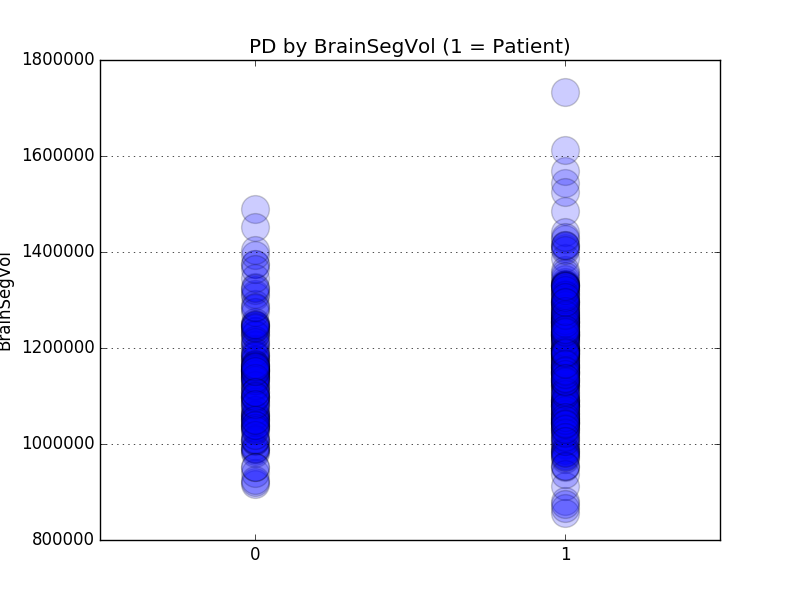
\includegraphics[width=0.5\textwidth]{Parkinson-distribution-BrainSegVol.png}\label{fig:f1}}
  \hfill
  \subfloat[]{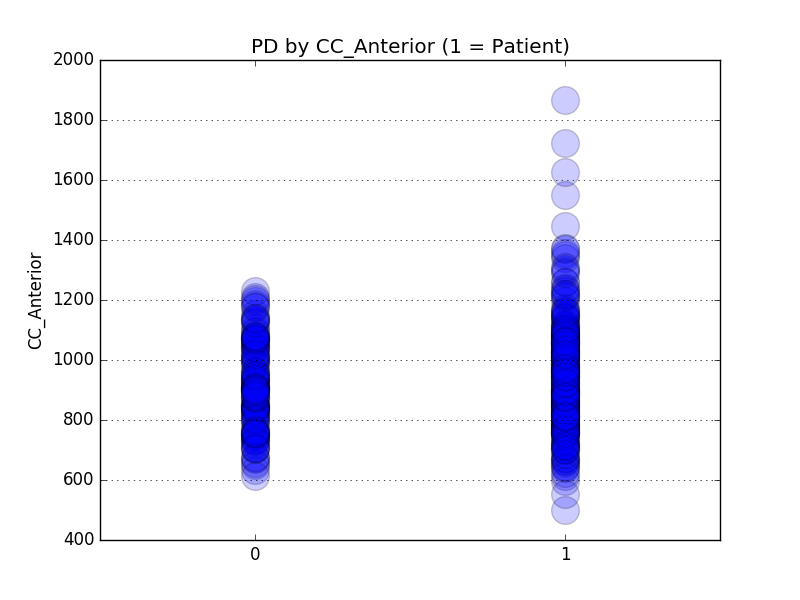
\includegraphics[width=0.5\textwidth]{Parkinson-distribution-CC_Anterior.png}\label{fig:f2}}
  \\
    \subfloat[]{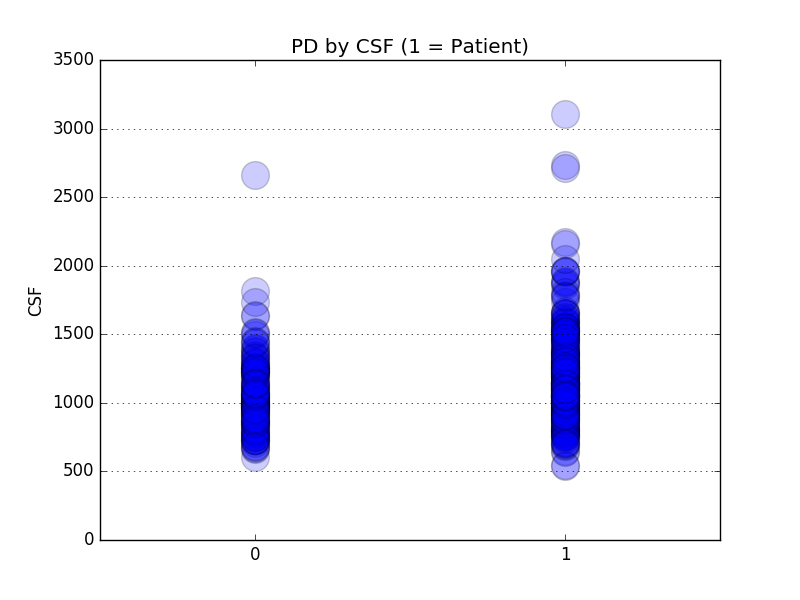
\includegraphics[width=0.5\textwidth]{Parkinson-distribution-CSF.png}\label{fig:f1}}
  \hfill
  \subfloat[]{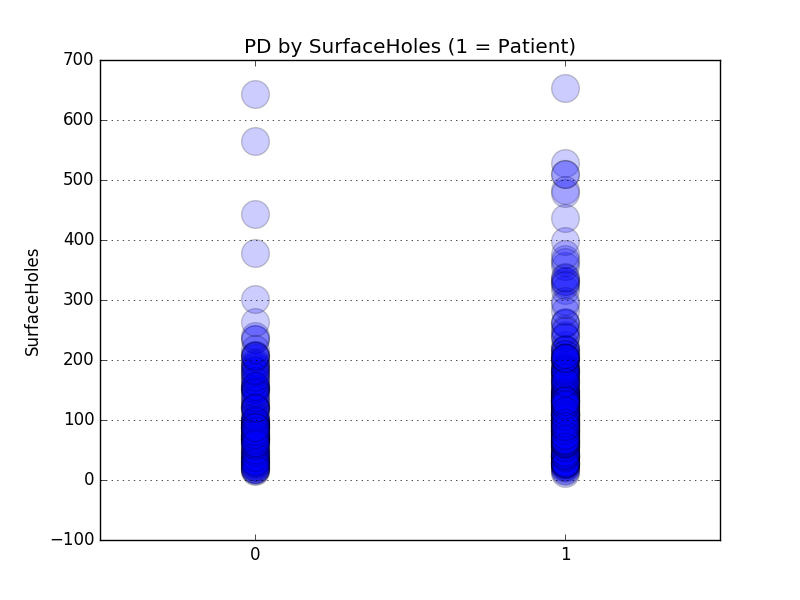
\includegraphics[width=0.5\textwidth]{Parkinson-distribution-SurfaceHoles.png}\label{fig:f2}}
  \caption{Data distributions in terms of the class labels and corresponding features; which are: (a) Brain segmented volume. (b) CC- Anterior. (c) CSF. (d) Surface holes.}\setlength{\belowcaptionskip}{0pt}
  \label{fig:feateval}
\end{figure}
Another set of evaluation is done over the extracted features. Data for every two features are plotted versus each other based on the corresponding class. Fig.\ref{fig:pairfeat} shows the distribution of data based on the two pair of features including $3rd$ ventricles vs lateral ventricles and $3rd$ ventricles vs. left vessels. In both of them, two features tend to have bigger value when the subject is PD.

\begin{figure}[!tbp]
  \centering
  \subfloat[]{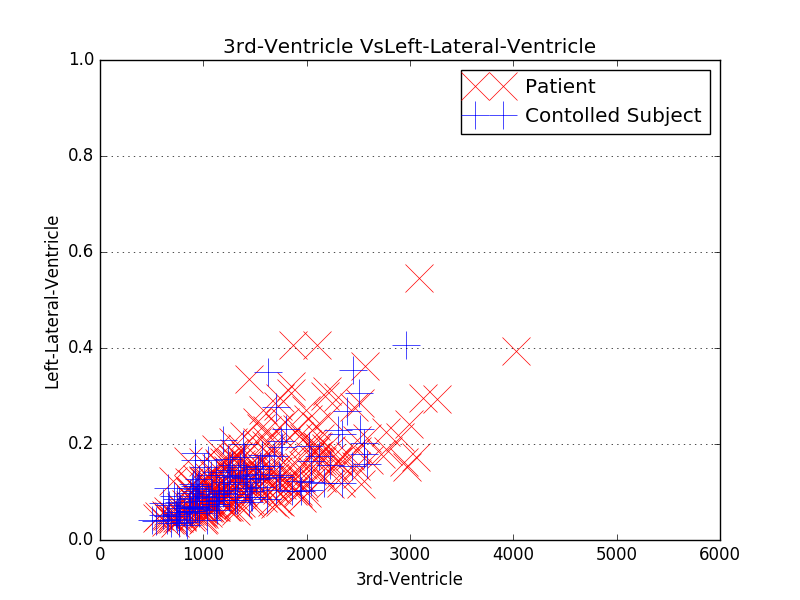
\includegraphics[width=0.5\textwidth]{3rd-Ventricle-Left-Lateral-Ventricle.png}\label{fig:f1}}
  \hfill
  \subfloat[]{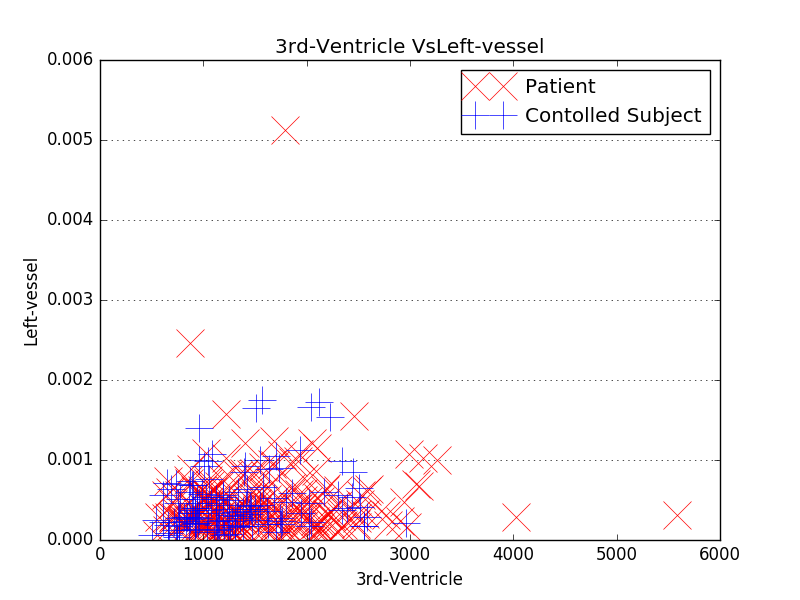
\includegraphics[width=0.5\textwidth]{3rd-Ventricle-Left-vessel.png}\label{fig:f2}}
  \caption{Data distribution based on the pair of features: (a)3rd ventricle and left lateral ventricle. (b) 3rd ventricle and left vessel.}
  \label{fig:pairfeat}
\end{figure}
As explained in the previous section, three types of classifiers are used in this study. These algorithm are run over $388$ samples with $141$ features. Internal and external cross validation is applied with $K=10$ for external and $k=5$ for internal (parameter tunning cross validation). The number of selected samples for the training part is $350$ and for the test part is $38$. Furthermore, the number of PD and HC in each group is presented in Table \ref{tab:trtedata}.
\begin{table}[h]\small
\centering
\caption{Data balance in training and testing parts.}\setlength{\abovecaptionskip}{0pt}
\begin{tabular}{|c|c|c|c|}
\hline
         & PD  & Hc  & Total \\ \hline
Training & 236 & 114 & 350   \\ \hline
Test     & 26  & 12  & 38    \\ \hline
\end{tabular}
\label{tab:trtedata}
\end{table}

As mentioned before, the classification algorithm needs a set of parameters for tunning which is selected as follow:
\begin{itemize}
\item logistic Regression (LR):\\
Regularization = $[1e-1, 1e-2, 1e-3, 1e-4, 1e-5]$, Tolerance = [1e-1, 1e-2, 1e-3, 1e-4, 1e-5]
\item Random Forest (RF):\\
Number of estimator =$[5, 10, 15, 20, 25]$, Max depth = $[2-10]$
\item Support Vector Machine (SVM): \\
C = $[0.1, 1, 10, 100, 1000]$, Gamma = $[10, 1, 1e-1, 1e-2, 1e-3, 1e-4]$, kernels = $[linear, rbf, poly]$
\end{itemize}
The evaluation metrics used in this paper for comparing the results of the classification algorithms include accuracy, confusion matrix (recall, precision) and AUC (area under ROC curve). The classification results for LR, RF and SVM are shown in Tables \ref{tab:logit}, \ref{tab:rf}, and \ref{tab:svm}, respectively.

\begin{table*}[h]\small
	\centering
	\caption{Logistic regression performance}
	\label{tab:logit}
	\csvautotabular{Logistic.csv}
\end{table*}

\begin{table*}[h]\small
	\centering
	\caption{Random forests performance}
	\label{tab:rf}
	\csvautotabular{RF.csv}
\end{table*}

\begin{table*}[h]\small
	\centering
	\caption{Support Vector Machine performance}
	\label{tab:svm}
	\csvautotabular{SVM.csv}
\end{table*}
Table \ref{tab:comp} shows the general comparison between these methods. The best result is for RF. In the table there are two sets of results related to using age/sex feature or doing the classification based only on the extracted volume based features from FreeSurfer.

Based on the literature review, most papers use VBM for data analysis and feature extraction. In this paper, one of the important goals was evaluating the FreeSurfer features for PD MRIs using machine learning techniques.  Generally, the experimental results show that the classification models need more information about the data that should be added to the current features, since these are low-level features and we need a set of high-level features as well. In future research, we are going to determine the useful general features that can be combined with the volume based extracted features.
\begin{table*}[h]\small
	\centering
	\caption{Comparing performance of different classifiers}
	\label{tab:comp}
	\csvautotabular{compmet.csv}
\end{table*}
\section{Conclusion}
We presented an automatic MRI based CAD system for diagnosing Parkinson’s Disease (PD) which is the second common neurodegenerative disease affecting elderly people. This disease is exposed by loss of neuro-transmitters that control body movements and there is no cure other than earlier diagnosis with better and more efficient treatment for patients. MR T1 images from the public PPMI PD data set is used. FreeSurfer is used for feature extraction and preprocessing. The decision model for classification of the extracted feature data is based on LR, RF and SVM methods. In the experimental results, the ability of these three types of classifiers for PD diagnosis are compared to each other. Results show that using only MRI is a potential option for PD diagnosis. This approach will avoid exposing the brain to harmful radiation based scans. In future work, the efficiency of the proposed method could be improved by adding high level features to the current ones. The classification rate with MRI needs to be improved to get close to those using raditation based scanning.
\begin{thebibliography}{4}

\bibitem{1} https://parkinsonsnewstoday.com/parkinsons-disease-statistics/.

\bibitem{2} S.H. Fox, R. Katzenschlager, S.Y. Lim, B. Ravina, K. Seppi, M. Coelho, W. Poewe,
O. Rascol, C.G. Goetz, C. Sampaio, The movement disorder society
evidence-based medicine review update: treatments for the motor symptoms
of Parkinson’s disease, Mov. Disord. 26 (S3) (2011) S2–S41.


\bibitem{3} K.R. Chaudhuri, A.H. Schapira, Non-motor symptoms of Parkinson’s disease:
dopaminergic pathophysiology and treatment, The Lancet Neurology 8 (5)
(2009) 464–474.

\bibitem{4} Rana, B., Juneja, A., Saxena, M., Gudwani, S., Kumaran, S., Behari, M. and Agrawal, R. (2017). Relevant 3D local binary pattern based features from fused feature descriptor for differential diagnosis of Parkinson’s disease using structural MRI. Biomedical Signal Processing and Control, 34, pp.134-143.

\bibitem{5}  Adeli, E. et al. Joint feature-sample selection and robust diagnosis of parkinson’s disease from MRI data. NeuroImage 141, 206–219 (2016).

\bibitem{6} Prashanth, R., Roy, S. D., Mandal, P. K., and Ghosh, S., Automatic classification and prediction models for early Parkinson’s disease diagnosis from SPECT imaging. Expert Syst. Appl. 41:3333–3342, 2014.

\bibitem{7} Marios Politis and Clare Loane, “Serotonergic Dysfunction in Parkinson's Disease and Its Relevance to Disability,” TheScientificWorldJOURNAL, vol. 11, Article ID 172893, 9 pages, 2011.

\bibitem{8} N.K. Focke, G. Helms, S. Scheewe, P.M. Pantel, C.G. Bachmann, P. Dechent, J.
Ebentheuer, A. Mohr, W. Paulus, C. Trenkwalder, Individual voxel-base subtype prediction can differentiate progressive supranuclear palsy from idiopathic parkinson syndrome and healthy controls, Hum. Brain Mapp. 32 (11) (2011) 1905–1915.

\bibitem{9} G.S. Babu, S. Suresh, B.S. Mahanand, A novel PBL-McRBFN-RFE approach for identification of critical brain regions responsible for Parkinson’s disease, Expert Syst. Appl. 41 (2) (2014) 478–488.

\bibitem{10} C. Salvatore, A. Cerasa, I. Castiglioni, F. Gallivanone, A. Augimeri, M. Lopez, G. Arabia, M. Morellie, M.C. Gilardic, A. Quattrone, Machine learning on brain MRI data for differential diagnosis of Parkinson’s disease and Progressive Supranuclear Palsy, J. Neurosci. Methods 222 (2014) 230–237.

\bibitem{11} B. Rana, A. Juneja, M. Saxena, S. Gudwani, S.K. Senthil, R. Agrawal, M. Behari, Regions-of-interest based automated diagnosis of Parkinson’s disease using T1-weighted MRI, Expert Syst. Appl. 42 (9) (2015) 4506–4516.

\bibitem{12} B. Rana, A. Juneja, M. Saxena, S. Gudwani, S.K. Senthil, M. Behari, R.K. Agrawal, Graph-theory-based spectral feature selection for computer aided diagnosis of Parkinson’s disease using T1-weighted MRI, Int. J. Imaging Syst. Technol. 25 (3) (2015) 245–255.

\bibitem{13} Bo Peng, Suhong Wang, Zhiyong Zhou, Yan Liu, Baotong Tong, Tao Zhang, Yakang Dai, A multilevel-ROI-features-based machine learning method for detection of morphometric  biomarkers in Parkinson’s disease, Neuroscience Letters, Volume 651,2017, Pages 88-94, ISSN 0304-3940.

\bibitem{14} Adeli, E., Shi, F., An, L., Wee, C. Y., Wu, G., Wang, T., \& Shen, D. (2016). Joint feature-sample selection and robust diagnosis of Parkinson's disease from MRI data. NeuroImage, 141, 206-219.

\bibitem{15} https://ida.loni.usc.edu/home.

\bibitem{16} https://surfer.nmr.mgh.harvard.edu/fswiki.

\bibitem{f}  A.  Worker  and et al. Cortical  thickness,  surface  area  and  volume  measures  in  parkinson’s  disease, multiple system atrophy and progressive supranuclear palsy. PLOS ONE, 9(12), 2014.

\bibitem{LR} Peng, Chao-Ying Joanne, et al. “An Introduction to Logistic Regression Analysis and Reporting.” The Journal of Educational Research, vol. 96, no. 1, 2002, pp. 3–14.

\bibitem{17} J. Martin and D. Jurafsky, Speech and language processing.Prentice, Hall, 2000.



\bibitem{18} L. Breiman. Random forests. Machine learning, 45(1):5–32, 2001.

\bibitem{19} V. Vapnik, The Nature of Statistical Learning Theory, Springer-Verlag, New York, 1995.

\end{thebibliography}


% \section*{Appendix: Springer-Author Discount}

% LNCS authors are entitled to a 33.3\% discount off all Springer
% publications. Before placing an order, the author should send an email,
% giving full details of his or her Springer publication,
% to \url{orders-HD-individuals@springer.com} to obtain a so-called token. This token is a
% number, which must be entered when placing an order via the Internet, in
% order to obtain the discount.

\end{document}
